% ============================================================
% COPYWRITING 360° — Okładka
% Kompilacja: xelatex cover.tex
% ============================================================
\documentclass{article}
\usepackage[paperwidth=210mm, paperheight=302mm, margin=0pt]{geometry}
\usepackage{tikz}
\usetikzlibrary{calc,positioning}
\usepackage{fontspec}
\usepackage{xcolor}
\pagestyle{empty}
\parindent=0pt
\topskip=0pt

% --- Kolory ---
\definecolor{primaryblue}{HTML}{1a73e8}
\definecolor{primarydark}{HTML}{0d47a1}
\definecolor{deepnavy}{HTML}{0a1628}
\definecolor{midnavy}{HTML}{112240}
\definecolor{accentgreen}{HTML}{00c853}
\definecolor{accentcyan}{HTML}{00b8d4}
\definecolor{primarylight}{HTML}{e3f2fd}
\definecolor{textmuted}{HTML}{8892b0}

% --- Fonty ---
\setmainfont{Liberation Sans}
\setsansfont{Liberation Sans}

\begin{document}%
\vspace*{-\baselineskip}%
\noindent\resizebox{\paperwidth}{\paperheight}{%
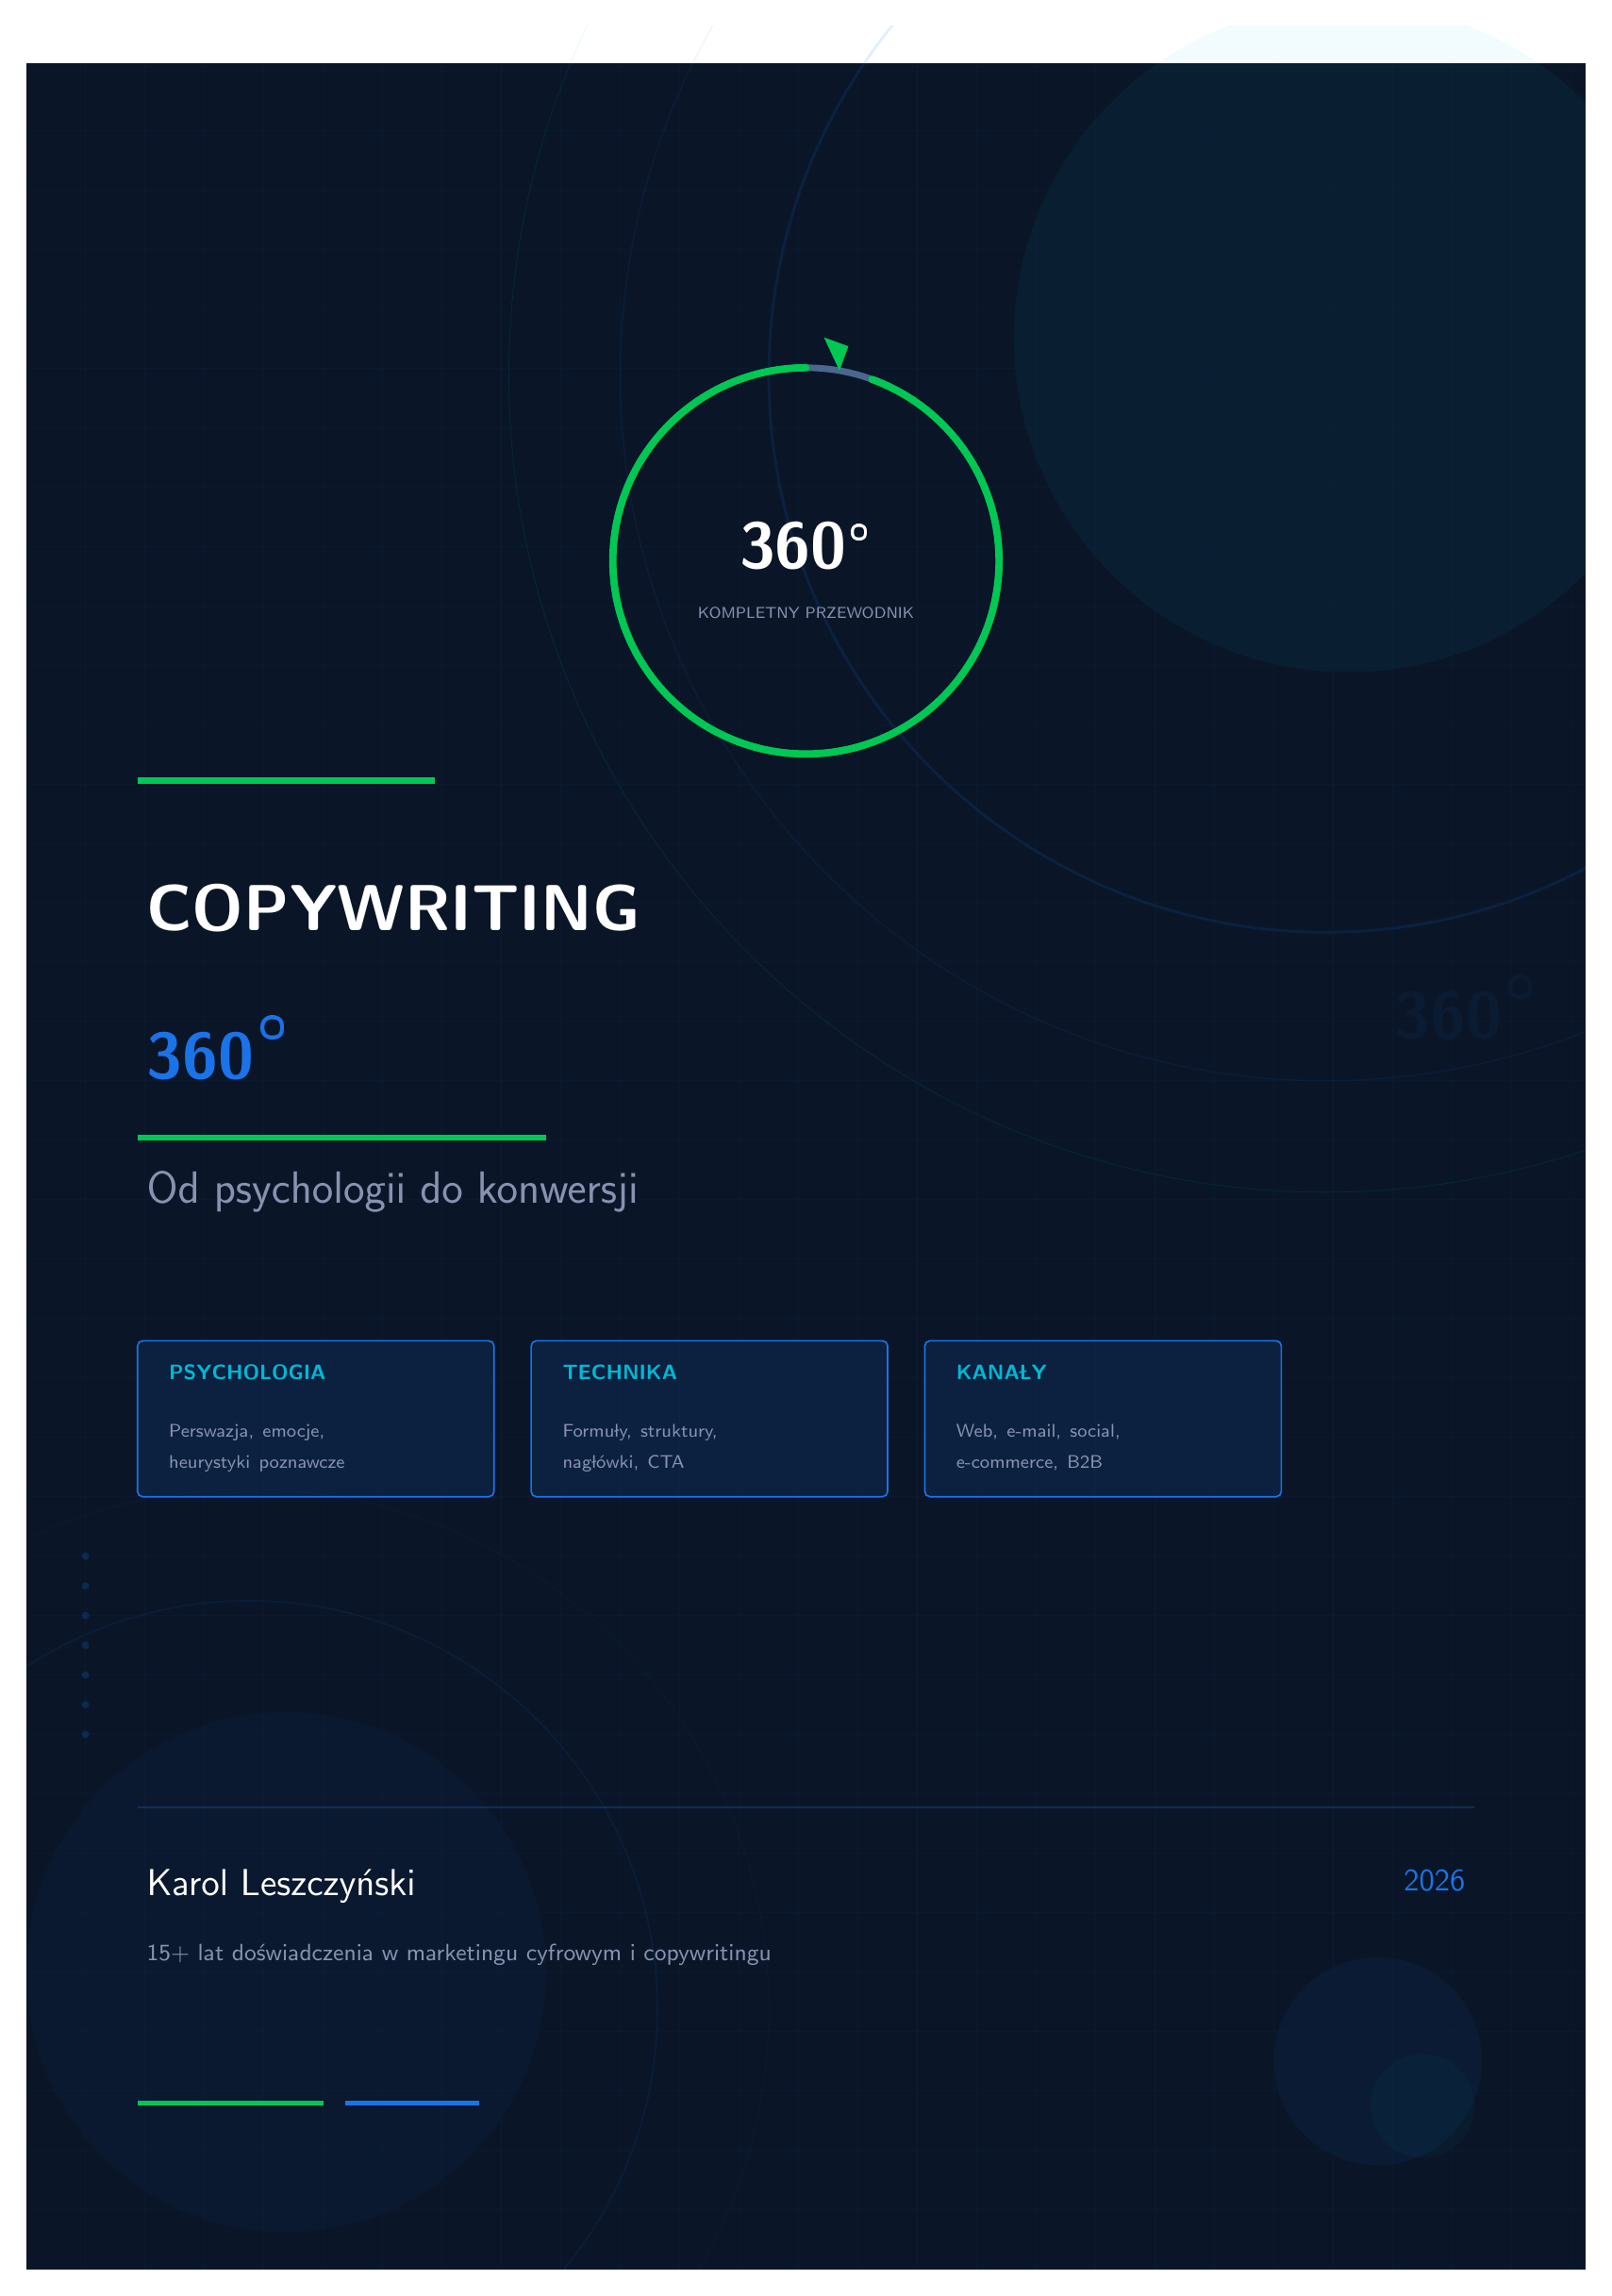
\begin{tikzpicture}[x=1mm, y=1mm]

% === Wymiary ===
\useasboundingbox (0,0) rectangle (210,302);
\clip (0,0) rectangle (210,302);

% === TŁO ===
\fill[deepnavy] (0,0) rectangle (210,297);

% === Subtelna siatka ===
\begin{scope}[opacity=0.035]
  \foreach \x in {0,8,...,210} {
    \draw[primaryblue, line width=0.2pt] (\x, 0) -- (\x, 297);
  }
  \foreach \y in {0,8,...,297} {
    \draw[primaryblue, line width=0.2pt] (0, \y) -- (210, \y);
  }
\end{scope}

% === Geometryczne koła — prawy górny róg ===
\draw[primaryblue, line width=1pt, opacity=0.12]
  (175, 255) circle (75);
\draw[primaryblue, line width=0.5pt, opacity=0.08]
  (175, 255) circle (95);
\draw[accentcyan, line width=0.3pt, opacity=0.10]
  (175, 255) circle (110);

% Koła — lewy dolny
\draw[primaryblue, line width=0.6pt, opacity=0.08]
  (30, 35) circle (55);
\draw[primaryblue, line width=0.3pt, opacity=0.05]
  (30, 35) circle (70);

% === Poświata ===
\fill[accentcyan, opacity=0.05] (178, 260) circle (45);
\fill[primaryblue, opacity=0.04] (35, 40) circle (35);

% === Duże "360°" w tle ===
\node[anchor=east, opacity=0.055] at (205, 170) {%
  \fontsize{170}{170}\selectfont\bfseries\sffamily\color{primaryblue}%
  360\textdegree%
};

% === Kółko z 360° — wyróżniony element graficzny ===
\draw[primaryblue!50, line width=2.5pt, opacity=0.5]
  (105, 230) circle (26);
\draw[accentgreen, line width=2.8pt, line cap=round]
  (105, 230) ++(90:26) arc (90:430:26);
% Grot strzałki
\fill[accentgreen]
  ([shift={(80:26)}]105,230) -- ++(70:3.5) -- ++(160:3.5) -- cycle;
% Tekst wewnątrz
\node[anchor=center] at (105, 232) {%
  \fontsize{26}{26}\selectfont\bfseries\sffamily\color{white}%
  360\textdegree%
};
\node[anchor=center] at (105, 223) {%
  \fontsize{6.5}{6.5}\selectfont\sffamily\color{textmuted}%
  KOMPLETNY PRZEWODNIK%
};

% === Linia akcentowa ===
\fill[accentgreen] (15, 200) rectangle (55, 200.8);

% === TYTUŁ ===
\node[anchor=south west] at (15, 179) {%
  \fontsize{44}{48}\selectfont\bfseries\sffamily\color{white}%
  COPYWRITING%
};
\node[anchor=south west] at (15, 159) {%
  \fontsize{44}{48}\selectfont\bfseries\sffamily\color{primaryblue}%
  360\textdegree%
};

% === PODTYTUŁ ===
\fill[accentgreen] (15, 152) rectangle (70, 152.7);
\node[anchor=north west] at (15, 149) {%
  \fontsize{16}{20}\selectfont\sffamily\color{textmuted}%
  Od psychologii do konwersji%
};

% === TRZY FILARY — boxy tematyczne ===
% Filar 1 — Psychologia
\fill[primaryblue, opacity=0.12, rounded corners=2pt]
  (15, 104) rectangle (63, 125);
\draw[primaryblue, line width=0.6pt, rounded corners=2pt]
  (15, 104) rectangle (63, 125);
\node[anchor=north west] at (18, 123) {%
  \fontsize{8}{8}\selectfont\bfseries\sffamily\color{accentcyan}%
  PSYCHOLOGIA%
};
\node[anchor=north west, text width=40mm] at (18, 115) {%
  \fontsize{7}{9}\selectfont\sffamily\color{textmuted}%
  Perswazja, emocje,\\heurystyki poznawcze%
};

% Filar 2 — Technika
\fill[primaryblue, opacity=0.12, rounded corners=2pt]
  (68, 104) rectangle (116, 125);
\draw[primaryblue, line width=0.6pt, rounded corners=2pt]
  (68, 104) rectangle (116, 125);
\node[anchor=north west] at (71, 123) {%
  \fontsize{8}{8}\selectfont\bfseries\sffamily\color{accentcyan}%
  TECHNIKA%
};
\node[anchor=north west, text width=40mm] at (71, 115) {%
  \fontsize{7}{9}\selectfont\sffamily\color{textmuted}%
  Formuły, struktury,\\nagłówki, CTA%
};

% Filar 3 — Kanały
\fill[primaryblue, opacity=0.12, rounded corners=2pt]
  (121, 104) rectangle (169, 125);
\draw[primaryblue, line width=0.6pt, rounded corners=2pt]
  (121, 104) rectangle (169, 125);
\node[anchor=north west] at (124, 123) {%
  \fontsize{8}{8}\selectfont\bfseries\sffamily\color{accentcyan}%
  KANAŁY%
};
\node[anchor=north west, text width=40mm] at (124, 115) {%
  \fontsize{7}{9}\selectfont\sffamily\color{textmuted}%
  Web, e-mail, social,\\e-commerce, B2B%
};

% === Dekoracyjne kropki (lewa krawędź) ===
\foreach \y in {72,76,...,96} {
  \fill[primaryblue, opacity=0.2] (8, \y) circle (0.5);
}

% === SEPARATOR ===
\fill[primaryblue, opacity=0.25] (15, 62) rectangle (195, 62.3);

% === AUTOR ===
\node[anchor=north west] at (15, 55) {%
  \fontsize{15}{15}\selectfont\sffamily\color{white}%
  Karol Leszczyński%
};
\node[anchor=north west] at (15, 45) {%
  \fontsize{9}{9}\selectfont\sffamily\color{textmuted}%
  15+ lat doświadczenia w marketingu cyfrowym i copywritingu%
};

% === ROK ===
\node[anchor=north east] at (195, 55) {%
  \fontsize{13}{13}\selectfont\sffamily\color{primaryblue}%
  2026%
};

% === Dolne paski akcentowe ===
\fill[accentgreen] (15, 22) rectangle (40, 22.7);
\fill[primaryblue] (43, 22) rectangle (61, 22.7);

% === Dekoracja — prawy dół ===
\fill[primaryblue, opacity=0.06] (182, 28) circle (14);
\fill[accentcyan, opacity=0.04] (188, 22) circle (7);

\end{tikzpicture}%
}%
\end{document}